\begin{figure*}[ht]
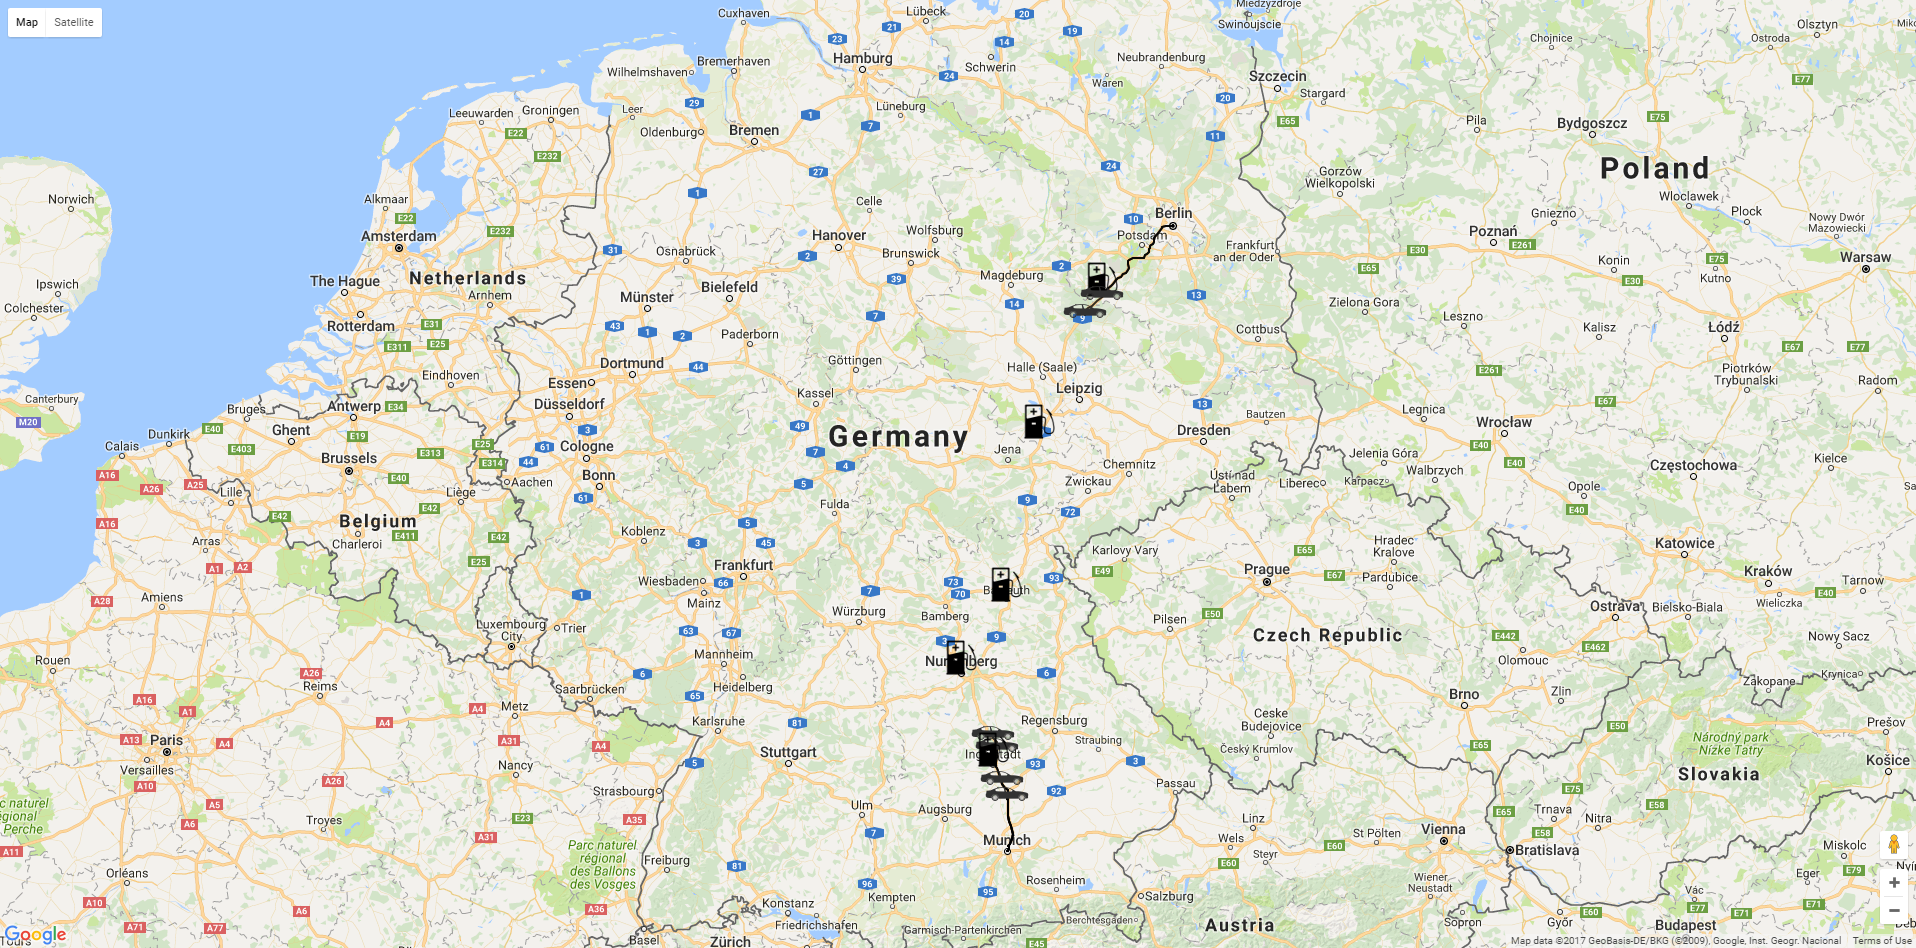
\includegraphics[width=\textwidth]{simulation_manager}
\caption{Simulation Manager Interface}
\end{figure*}

\newpage


\section{Simulation Manager Interface}

\subsection{Approach}

The Simulation Manager Interface is supposed to be a frontend for a traffic simulation framework that simulates electric vehicles on a highway and optimizes their travel time. The actual simulation and calculation of all relevant data thus happens in the backend. The purpose of the frontend is to assist the person running the simulation, i.e. the simulation manager.

Without a visual representation of the simulation, it is very challenging for the simulation manager to understand the current state and behavior of the simulation since humans are naturally not very good at interpreting large amounts of data at a high speed.

Our approach for the implementation of the prototype is to display the simulation data on a map. The two main components that need to be integrated into the map are the electric vehicles (EVs) and charging stations (CSs).

We decided to use the Google Maps JavaScript API as a foundation for the implementation since it provides a lot of assistance in setting up the functionality we will need, e.g. good map data, zoom capability, marker positioning, info panels and so on. Additionally, almost everyone is already familiar with using the Google Maps UI, which is another important advantage.

The project structure follows guiding principles that are commonly applied in modern frontend web development, such as the clear seperation of markup, functionality, style, assets, and data.


\subsection{Structure}

The project structure of the Simulation Manager Interface can easily be inferred by taking a look at the directory tree diagram:

\vspace{2mm}
\setlength{\DTbaselineskip}{11pt}
\dirtree{%
.1 /.
.2 css.
.3 main.css.
.2 data.
.3 cs.json.
.3 ev.json.
.2 img.
.3 markers.
.4 battery.png.
.4 car.png.
.2 js.
.3 config.js.
.3 cs.js.
.3 ev.js.
.3 main.js.
.3 map.js.
.2 less.
.3 main.less.
.3 map.less.
.2 index.html.
}
\vspace{2mm}

The reason for sticking to this conventional structure is that it facilitates the future maintenance of the project by developers that were not part of its original development.


\subsection{Markup}

The HTML markup needed to get our Simulation Manager Interface to show is minimal.

We set the page title to ``EV Traffic Simulation'', link the generated css stylesheet, the newest miminized jQuery version from a CDN, the Google Maps JavaScript API script with our API key attached at the end of the url, and finally the javascript files of our project.

\begin{minted}{html}
<!doctype html>

<html lang="en">
<head>
    <title>EV Traffic Simulation</title>

    <link rel="stylesheet" href="css/main.css">

    <!-- jQuery CDN -->
    <script src="https://code.jquery.com/jquery-3.1.1.min.js">
    </script>

    <!-- Google Maps JavaScript API -->
    <script src="https://maps.googleapis.com/maps/api/js?key=.">
    </script>

    <!-- Configuration Options -->
    <script src="js/config.js"></script>

    <!-- Electric Vehicle Model -->
    <script src="js/ev.js"></script>

    <!-- Charging Station Model -->
    <script src="js/cs.js"></script>

    <!-- Google Map Wrapper -->
    <script src="js/map.js"></script>

    <!-- Main Application Script -->
    <script src="js/main.js"></script>
</head>

<body>
    <div id="map"></div>
</body>
</html>
\end{minted}

The document body merely consists of a \texttt{div} with the id \texttt{map}. Everything else is either style or functionality that is outsourced to css or javascript files, respectively.

\newpage
\subsection{Configuration}

The settings of the Simulation Manager Interface can be found in \texttt{js/config.js}.

\begin{minted}{javascript}
var config = {
    mapID: "map",
    mapCenter: "Germany",
    mapZoom: 7,
    markers: {
        car: {
            url: "img/markers/car.png",
            anchor: new google.maps.Point(24, 18)
        },
        battery: {
            url: "img/markers/battery.png",
            anchor: new google.maps.Point(20, 36)
        }
    }
};
\end{minted}

Below is a short explanation of the various configuration parameters:

\begin{table}[htp]
\renewcommand{\arraystretch}{1.9}
\begin{tabular}{p{1.8cm}p{5.6cm}}
\texttt{mapID} & The \texttt{id} attribute of the HTML element in which the map should be rendered.\\
\texttt{mapCenter} &  The map will be aligned to show this location at its center. Geocoding to retrieve the coordinates from the location name is performed by the Google Maps JavaScript API.\\
\texttt{mapZoom} &  The initial zoom level of the map. The value \texttt{0} corresponds to a map of the Earth that is fully zoomed out, while a value of 20 shows buildings in detail \cite{google-api-zoom}. The parameter must be an integer.\\
\texttt{markers} & The small graphics that need to be displayed on the map. The object \texttt{markers["car"]} is used for the EVs and \texttt{markers["battery"]} for the charging stations.
\newline\newline
The \texttt{url} property of the image is given relative to the project directory. The anchor attribute lets you control which point of the image will be placed at the object's actual pixel coordinates.
\end{tabular}
\vspace{4mm}
\caption{Simulation Manager Interface: Configuration Options}
\end{table}


\newpage
\subsection{Application}

The main application routine consists of constructing an instance \texttt{map} of our \texttt{Map} function, creating empty lists that will hold the electric vehicles (EVs) and charging stations (CSs), and finally creating those EVs and CSs with certain parameters.

The constructor of function \texttt{Map} does not need any arguments. Since there is only one map at a time, those settings are controlled via the project-wide \texttt{config.js} file instead.

\begin{minted}{javascript}
$(document).ready(function () {

    // Init map
    var map = new Map();

    // Electric vehicles traveling from A to B
    var ev = [];

    ev.push(
      new EV(map.map, 1,  0, "Munich", "Berlin"));

    ev.push(
      new EV(map.map, 2, 10, "Munich", "Berlin"));

    ev.push(
      new EV(map.map, 3,  0, "Berlin", "Munich"));

    ev.push(
      new EV(map.map, 4, 15, "Berlin", "Munich"));

    // Charging stations at location C
    var cs = [];

    cs.push(new CS(map.map, 1, "Ingolstadt"));
    cs.push(new CS(map.map, 2, "Nuremberg"));
    cs.push(new CS(map.map, 3, "Bayreuth"));
    cs.push(new CS(map.map, 4, "Osterfeld"));
    cs.push(new CS(map.map, 5, "Rabenstein"));
});
\end{minted}

The \texttt{EV} constructor needs a Google Maps JavaScript API map object, which \texttt{map.map} is, an id, a starting delay in seconds, an initial location and a target location.

The constructor \texttt{CS} for charging stations needs the same two arguments as the \texttt{EV} constructor and its location. The geocoding of the location string to the actual coordinates is done via the Google Maps API.


\subsection{Map}

The \texttt{Map} function is merely a wrapper around the Google Map object and automatically takes care of its initialization upon construction.

This is done by calling its own init function directly in its function body. The \texttt{google.maps.Map} object constructor takes two arguments: The HTML element in which the newly created map should be rendered in and optionally a \texttt{MapOptions} object which allows to selectively alter map configuration options.

In our case, we supply the first argument via retrieving the container element by its identifier as it is specified in our config file as \texttt{mapID}. Additionally, we do supply a \texttt{MapOptions} literal as our second argument to change the map type to \texttt{ROADMAP}, which is the obvious map type choice for our use case of running a traffic simulation.

\begin{minted}{javascript}
function Map() {
  this.init = function () {

    // Create new Google Map
    this.map = new google.maps.Map(
      document.getElementById(config.mapID),
      {
        mapTypeId: google.maps.MapTypeId.ROADMAP
      }
    );

    // Center and fit country in viewport
    var geocoder = new google.maps.Geocoder();
    var map = this.map;

    geocoder.geocode({'address': config.mapCenter},
      function (results, status) {
        if (status == google.maps.GeocoderStatus.OK) {
          map.setCenter(results[0].geometry.location);
          map.fitBounds(results[0].geometry.viewport);
        }
    });
  };

  this.init();
}
\end{minted}

After having created our \texttt{map} object, we construct a \texttt{geocoder} via the API. Geocoding refers to the process of translating an address in string format to a location given in coordinates. A geocoder is the software entity that performs this action.

The \texttt{geocode} function is used to do exactly that: We supply \texttt{config.mapCenter} from our settings as the address, which is the string ``Germany'' in our case, and an anonymous function that gets called with the result of the geocoding process. If \texttt{status} equals \texttt{OK}, the geocoding was performed successfully and \texttt{results} contains meaningful information about the location.

Via the functions \texttt{setCenter} and \texttt{fitBounds}, we position the map with the location returned for Germany at its center and make sure that the area fits within the viewport. Internally, this determines the highest zoom level such that the area is still completely contained within the viewport.


\subsection{Charging Station}

The attributes and functionality of a charging station are encapsuled by the function \texttt{CS}. It takes three arguments: The Google Map object, an id and a location.

The attribute \texttt{stats} holds the information that will be supplied by the simulation framework during the traffic simulation. The frontend is responsible for displaying this data in a reasonable way, such that the simulation manager can get a good idea of what is happening at any time.

\begin{minted}{javascript}
function CS(map, id, location) {
    var CS = this;

    var stats = {
        id: id,
        time: '',
        queue_length: '',
        busy_poles_fc: '',
        busy_poles_tsc: '',
        arrived_cars: '',
        leaving_cars: '',
        queued_cars: '',
        plugged_cars: '',
        energy_consumed: '',
        energy_produced: '',
        energy_stored: '',
        energy_bought: '',
        queue_prediction_fc: '',
        queue_prediction_tsc: ''
    };

    var schedule = [
        {
            id: 1,
            data: {
                ev: '',
                start: '',
                duration: '',
                charging_technology: '',
                binding: '',
                confirmed: ''
            }
        }
    ];
\end{minted}

For a charging station, this is for example its queue length, the number of busy poles of certain types, the number of arriving and leaving cars, information on its energy consumption and production, and so on.

The attribute \texttt{schedule} contains information regarding the state of the scheduling system of the respective charging station. It is a list of scheduling entries which possess an id and other necessary information about the booking.

The \texttt{init} function of a charging station is responsible for adding itself onto the map and creating a panel that contains the technical information.

In order to get the charging station to show on the map, a \texttt{Marker} object needs to be created. It has only one optional argument which is a \texttt{MarkerOptions} object. We use it to specify the map to which the marker should be added (the Google Map object \texttt{map} was passed in the \texttt{CS} constructor) and the icon that should function as its visual representation, which is a battery symbol that was added via the config file.

Finally, we use our helper function \texttt{setPosition} to place the created marker at the location that was supplied during the construction of the charging station.

\begin{minted}{javascript}
    this.init = function () {
        var marker = new google.maps.Marker({
            map: map,
            icon: config.markers.battery
        });

        CS.setPosition(marker);

        var panel = new google.maps.InfoWindow({
            content: CS.getStats()
        });

        CS.initStats(panel, marker);
    };
\end{minted}

Afterwards, an \texttt{InfoWindow} object is created which is a panel that should toggle its visibility upon clicking on the associated marker. The only data we need to supply is its content which is HTML code in string format. The helper function \texttt{getStats} takes care of formatting the attributes of the charging station.

The function \texttt{initStats} takes the panel and marker as its arguments. It is needed to establish the connection between the two, such that the panel opens and closes when the marker is clicked.

\begin{minted}{javascript}
    this.setPosition = function (marker) {
        var geocoder = new google.maps.Geocoder();

        geocoder.geocode({'address': location},
          function (results, status) {
            if (status ==
                google.maps.GeocoderStatus.OK)
            {
               marker.setPosition(
                 results[0].geometry.location
               );
            }
        });
    };
\end{minted}

The functionality of the helper function \texttt{setPosition} is similar to what needed to be done during the map initialization.

Its purpose is to set the position of the marker, which is given as an argument and represents the charging station, on the map. In our prototype, the location of a charging station is given as an address in string format upon construction, which is why the function \texttt{geocode} is needed again to resolve the acutual coordinates.

Once the geocoding was successful, the function \texttt{setPosition} on the marker can be called with the result as its argument.

As outlined before, the function \texttt{initStats} connects \texttt{marker} with \texttt{pabel}. This is done by adding a listener on the \texttt{marker} objects that performs a certain function on the event 'click'. This function tells the panel to open at the position of the marker \texttt{this} on map \texttt{this.map}.

\begin{minted}{javascript}
    this.initStats = function (panel, marker) {
        marker.addListener('click', function () {
            panel.open(this.map, this);
        });
    };
\end{minted}

The function \texttt{updateStats} can be used to refresh the content of the info panel of the charging station. It takes the panel as its argument and calls the \texttt{setContent} function with the result of \texttt{getStats}.

\begin{minted}{javascript}
    this.updateStats = function (panel) {
        panel.setContent(CS.getStats());
    };
\end{minted}

The \texttt{getStats} function is used upon initialization and when updating the panel content.

Right now, it simply loops over the properties of attribute \texttt{stats} and concatenates their string representation with an HTML line break inbetween elements. In the future, this could easily be extended or modified to provide a better visual appearance.

\begin{minted}{javascript}
    this.getStats = function () {
        var info = '';

        for (var key in stats) {
            info += key + ': ' + stats[key] + '<br>';
        }

        return info;
    };
\end{minted}

As seen in the \texttt{map} function, the \texttt{init} function is automatically called upon construction of a charging station object:

\begin{minted}{javascript}
    this.init();
}
\end{minted}


\newpage
\subsection{Electric Vehicle}

The most important component of our simulation, the electric vehicle, is modelled by the \texttt{EV} function which takes four arguments: The Google Map object, an ID, a start time, an origin and a destination.

The parameter \texttt{start\_time} is used in our prototype to delay the vehicle's journey for a certain number of seconds starting at the beginning of the simulation. The parameters \texttt{origin} and \texttt{destination} are addresses in string format, such as cities or specific postal addresses.

The attributes \texttt{stats} and \texttt{schedule} serve the same function as they do in the charging station model. The simulation framework is expected to continuously fill these values in during the progress of the simulation. For an electric vehicle, the data contains information about its position, the distance and time travelled, the battery level, its speed and so on.

\begin{minted}{javascript}
function EV(map, id, start_time, origin, destination) {
    var EV = this;

    var stats = {
        id: id,
        time: '',
        position: '',
        geo_position: '',
        distance_travelled: '',
        time_travelled: '',
        time_waited: '',
        time_charged: '',
        time_driven: '',
        battery_level: '',
        speed: '',
        driving_flag: '',
        schedule_status: ''
    };

    var schedule =  [
        {
            id: 1,
            data: {
                station: '',
                km: '',
                target_soc: '',
                type: '',
                range: ''
            }
        }
    ];
\end{minted}

The \texttt{schedule} attribute is a list of charging stations that the smart scheduling algorithm used by the backend has determined for this vehicle to reach its destination as fast as possible. An entry contains the station id, the station's distance in kilometers and charging relevant information.

The function \texttt{start} requests a route to the EV's destination and animates the EV's marker along this route. In this prototype, Google's direction API is used to get a route from A to B. After the integration of the backend, the simulation framework would supply this route.

First, we construct a \texttt{DirectionsService} object. This is used to interact with Google's direction API. Then, we specify the request that will be send to Google. It contains the origin and destination that were handed over during the EV construction. They are both in string format. Additionally, we specify the travel mode by setting it to driving.

\begin{minted}{javascript}
    this.start = function () {
        var directions =
          new google.maps.DirectionsService();

        var request = {
            origin: origin,
            destination: destination,
            travelMode: google.maps.TravelMode.DRIVING
        };

        setTimeout(function () {
          directions.route(request,
            function (result, status) {
              if (status ==
                  google.maps.DirectionsStatus.OK)
              {
                EV.autoUpdate(
                  map, result.routes[0].legs
                );
              }
          });
        }, start_time * 1000);
    };
\end{minted}

Then, we use the function \texttt{route} with the arguments \texttt{request} and an anonymous function that will be called when the answer was received.

If \texttt{status} equals \texttt{OK}, the directions were successfully generated and \texttt{result} contains the route. The function \texttt{autoUpdate} is then used to start the animation of the vehicle along the route. It takes the Google map and the legs of the fastest route, i.e. the segments the route consists of.

The Javascript function \texttt{setTimeout} is used to delay the start of the animation by \texttt{start\_time} seconds from the beginning of the simulation.

The \texttt{autoUpdate} function is at the core of the simulation. It takes care of updating the EV's position. Therefore, it needs the Google map object and the legs of the route that was calculated.

The route can be shown on the map to signal where the vehicle has already travelled. It is represented by a \texttt{Polyline} that can be styled in different ways. In this case, it is a black line with opacity $0.8$ and weight $2$.

Then, a marker is created that represents the EV on the map. Its icon is specified in the settings as a car symbol. The EV also gets an info window analogous to the charging stations. Its content is the information that is stored in the attributes which is correctly formatted into HTML by \texttt{getStats}. Again, \texttt{initStats} establishes the connection between the marker and the panel, so that the info window opens when the marker was clicked.

\begin{minted}{javascript}
    this.autoUpdate = function (map, legs) {
        var route, marker, panel;

        route = new google.maps.Polyline({
            path: [],
            geodesic: true,
            strokeColor: '#000000',
            strokeOpacity: 0.8,
            strokeWeight: 2,
            editable: false,
            map: map
        });

        marker = new google.maps.Marker({
            map: map,
            icon: config.markers.car
        });

        panel = new google.maps.InfoWindow({
            content: EV.getStats()
        });

        EV.initStats(panel, marker);

        var timeUnit = 0;

        for (var i = 0;
             i < legs.length; i++) {
         for (var j = 0;
              j < legs[i].steps.length; j++) {
          for (var k = 0;
               k < legs[i].steps[j].path.length; k++) {
           setTimeout(
            function (coords) {

            route.getPath().push(coords);
            EV.moveMarker(map, marker, coords);
            EV.updateStats(panel);

            },
            50 * timeUnit++, legs[i].steps[j].path[k]
           );
          }
         }
        }
    };
\end{minted}

The triple loop construction is needed to iterate over the smallest segments of the route that is supplied by the Google directions API. The route consists of legs, which consist of steps, which consist of paths.

In the innermost loop, we take the coordinates of the current path as \texttt{coords}. They get pushed to the path of the route that is displayed on the map. Then, the EV's marker is moved to those coordinates via the helper function \texttt{moveMarker}. And finally, \texttt{updateStats} is used to reload the info panel content. The \texttt{setTimeout} function is used to achieve the animation effect. The nth path is travelled after $50n$ milliseconds. The variable \texttt{timeUnit} thus symbolizes one step.

The helper function \texttt{moveMarker} simply sets the position of the EV's marker to a certain coordinate that is given as \texttt{latlng}.

\begin{minted}{javascript}
    this.moveMarker = function (map, marker, latlng) {
        marker.setPosition(latlng);
    };
\end{minted}

In order to achieve the functionality that the info panel opens when the respective marker is clicked, a listener is added on the marker that calls the \texttt{open} function on the panel when the marker is clicked.

\begin{minted}{javascript}
    this.initStats = function (panel, marker) {
        marker.addListener('click', function () {
            panel.open(this.map, this);
        });
    };
\end{minted}

The helper function \texttt{updateStats} regenerates the EV information via \texttt{getStats} and sets the panel's content accordingly.

\begin{minted}{javascript}
    this.updateStats = function (panel) {
        panel.setContent(EV.getStats());
    };
\end{minted}

The \texttt{getStats} function works exactly the same as the one for the charging stations. The attribute \texttt{stats} is converted to an HTML string by concatenating the properties with line breaks inbetween.

\begin{minted}{javascript}
    this.getStats = function () {
        var info = "";

        for (var key in stats) {
            info += key + ": " + stats[key] + "<br>";
        }

        return info;
    };
\end{minted}

Finally, the \texttt{start} function is directly called as soon as the EV is constructed.

\begin{minted}{javascript}
    this.start();
}
\end{minted}


